\documentclass[sigplan,screen]{acmart}

\usepackage[ruled]{algorithm2e}
\usepackage{graphicx}
\usepackage{hyperref}

\graphicspath{ {./images/} }

\renewcommand{\algorithmcfname}{ALGORITHM}
%% Remove Permissions and ACM Reference Notes
\renewcommand\footnotetextcopyrightpermission[1]{}
\settopmatter{printacmref=false}
%%
%% \BibTeX command to typeset BibTeX logo in the docs
\AtBeginDocument{%
  \providecommand\BibTeX{{%
    \normalfont B\kern-0.5em{\scshape i\kern-0.25em b}\kern-0.8em\TeX}}}

\begin{document}

\title{Árvores Minimax para Jogos de Soma Zero}
\subtitle{DIM0806 - Estruturas de Dados e Algoritmos}

\author{Tiago Vinícius Remígio da Costa}
\email{vinicius.remigio@gmail.com}
\affiliation{
  \institution{DIMAp - Universidade Federal do Rio Grande do Norte}
  \city{Natal}
  \state{RN}
  \country{Brasil}
}

\begin{abstract}
  Árvores minimax têm sido usadas em conceitos de jogos de soma zero. 
  Neste trabalho veremos algumas implicações desta estrutura de dados, 
  assim como pseudo-código, complexidade, trade-offs e exemplos de utilização em problemas reais. 
  Além disso, será mostrado como exemplo uma implementação de exemplo usando o Jogo da Velha (Tic Tac Toe).
\end{abstract}

\keywords{algoritmos, estruturas de dados, árvores, teoria dos jogos, minimax, soma zero}

\maketitle
\pagestyle{plain}

\section{Introdução}
Este trabalho apresenta o algoritmo minimax \cite{russel2010} para jogos de soma zero. 
Obter algoritmos que calculem uma estratégia capaz de recomendar uma ação para qualquer estado. O algoritmo minimax é usado em tomada de decisões, encontrando uma jogada ótima para um jogador, assumindo que seu oponente também joga de forma ótima.
As demais seções são Funcionamento, incluindo Pseudocódigo e Complexidade, Trade-offs, Aplicações e por fim as Conclusões do trabalho.

\subsection{Soma Zero}
Em um jogo determinístico de soma zero, o placar final de um jogo em que dois jogadores são adversários.
para cada jogador pode ser vitória {\itshape(1 ponto)}, empate {\itshape(0 pontos)} ou derrota {\itshape(-1 ponto)}. 
Agentes jogadores possuem utilidades opostas. Isso permite que a função utilidade seja a mesma.

Além disso, os métodos de busca são sempre adversários, puramente competitivos, onde cada jogador está tentando ganhar e também provocando a derrota do oponente. O jogador que tenta ganhar é chamado de maximizador, tentando maximizar seu score, enquanto o oponente é chamado de minimizador, tentando minimizar o score do maximizador \cite{Aradhya01}.

Considerando essa premissa, o placar total deve ser sempre zero.
Cada jogador possui a informação completa, ou seja, tem a visão das jogadas realizadas pelo adversário. Os jogos são realizados em turno, ou seja, cada jogado possui a sua vez de jogar.

Muitos trabalhos com variações do minimax têm sido apresentados no decorrer dos anos na literatura \cite{Diderich93}

\section{Algoritmo Minimax}
Em uma busca minimax, a árvore representa o espaço de estados, onde os jogadores se alternam nos movimentos e o valor minimax é computado para cada nó, onde se busca a melhor utilidade contra um agente adversário ótimo, ou seja, a premissa é que o adversário jogue de forma racional
Para definir Minimax, necessitaremos de alguns conceitos.

A idéia do Minimax é determinar uma estratégia ótima para o jogador MAX e então decidir o melhor primeiro movimento.

Todos os estados possuem um valor associado, onde o maximizador realiza uma jogada para aumentá-lo e o minimizador realiza uma jogada para diminuí-lo. 
O valor é calculado através de uma heurística, chamada de função de utilidade.

\begin{itemize}
  \item{Estados: S, onde S0 é o estado inicial;}
  \item{Jogadores: P = {1...N}}
  \item{Ações: A}
  \item{Função de Transição: SxA -> S}
  \item{Teste de parada: S -> {t,f}}
  \item{Utilidades terminais: SxP -> R}
\end{itemize}

Solução par aum jogador é uma política: S -> A

\subsection{Passos do Minimax}

\begin{itemize}
  \item Gerar a árvore, da raíz até os estados terminais;
  \item Aplicar a função de utilidade para cada estado terminal para computar o valor;
  \item Usar a função de utilidade para determinar a utilidade dos nós um nível acima na árvore de busca;
  \item Calcular o valor dos nós filhos até a raíz, uma camada por vez;
  \item MAX escolhe o movimento que leva ao maior valor 
\end{itemize}

O movimento realizado é chamado de decisão minimax, por maximizar a utilidade sob a premissa que o oponente jogará para minimizá-lo perfeitamente.

\subsection{Pseudo-código}
O pseudocódigo do algoritmo Minimax segue como na imagem abaixo. 
\footnote{A implementação do algoritmo pode ser encontrada em \href{https://bit.ly/3jc3wH0}{https://bit.ly/3jc3wH0}}
As funções {\itshape minValue} e {\itshape maxValue} possuem o mesmo funcionamento, apenas invertendo a lógica.


\begin{algorithm}
\DontPrintSemicolon
  \caption{Algoritmo Minimax}
  \label{alg:generator}
  \SetKwProg{minimax}{Function \emph{minimax}}{}{end}
  \minimax{Object state}{
    \If{ state $s$ is final}{
        \Return{$s$}\;
    }
    minValue($s$)\;
    maxValue($s$)\;
  }

  \SetKwProg{maxValue}{maxValue}{}{}
  \maxValue{$s$}{
    init v = -inf\;
    \ForEach{successor in s}{
      v = max(v, value(successor))\;
    }
    \KwRet{v}\;
  }

  \SetKwProg{minValue}{minValue}{}{}
  \minValue{$s$}{
    init v = +inf\;
    \ForEach{successor in s}{
      v = min(v, value(successor))\;
    }
    \KwRet{v}\;
  }
\end{algorithm}

Na figura abaixo segue a árvore minimax gerada pelo algoritmo descrito. 
Para simplificar a visualização, o estado inicial considerado {\itshape(Depth 0)} já possui algumas jogadas.
A melhor decisão que o algoritmo retorna, ou seja, maximizando o valor para o jogador MAX é marcar a posição (2,2) do tabuleiro com X.

\begin{figure}[h]
  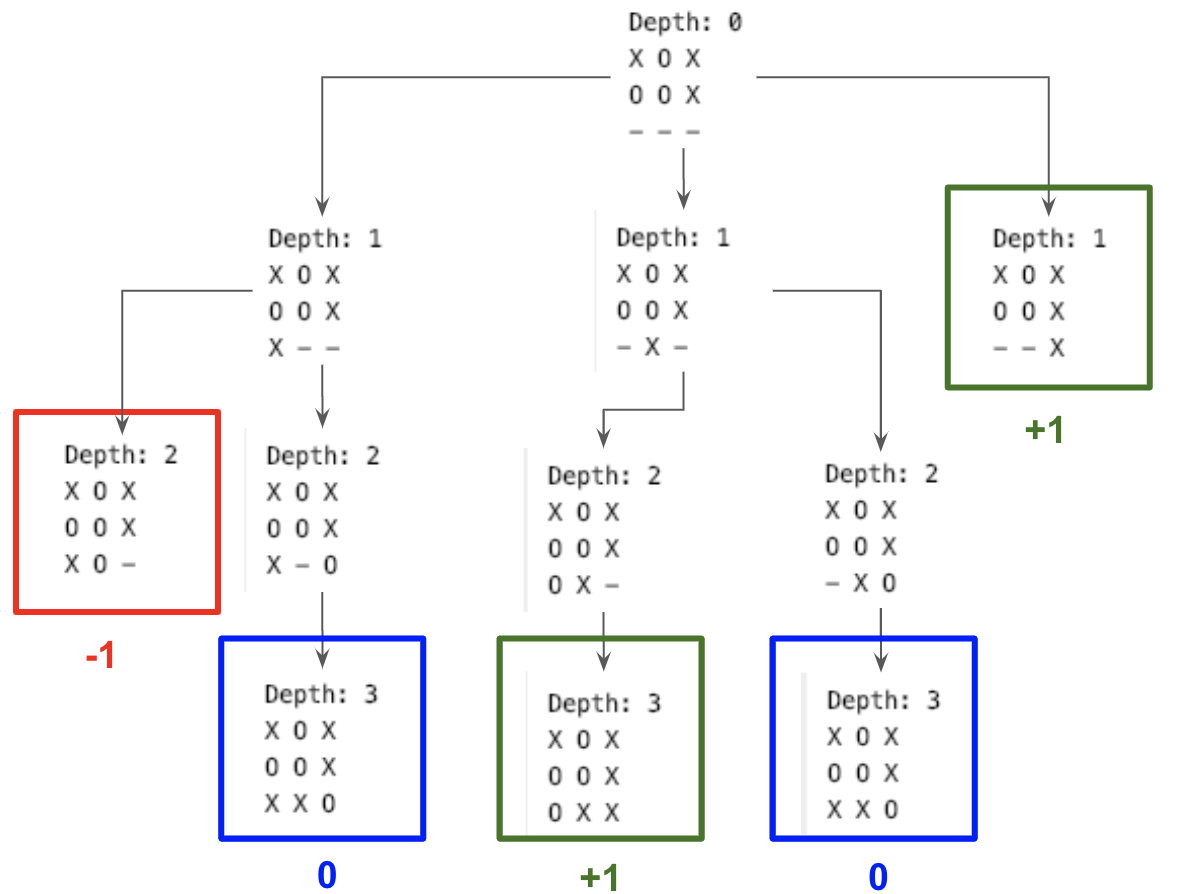
\includegraphics[width=8cm]{minimax_tree_1.png}
  \caption{Árvore MiniMax para um jogo da Velha, dado um estado inicial}
\end{figure}

\subsection{Complexidade}

Possui a mesma complexidade que a busca em profundidade {\itshape (depth-first search)}, tornando inviável quando a árvore é profunda.
Considerando que m é a profundidade máxima da árvore e b é a quantidade de movimentos válidos em cada ponto, temos que:
\begin{itemize}
  \item Complexide de tempo: $O(b^m)$
  \item Complexidade de espaço: $O(bm)$
\end{itemize}

Em termos práticos, esta complexidade de tempo é impraticável. Para isso, técnicas de poda são necessárias ao se trabalhar como representação Minimax, como será mostrado na próxima seção.

\section{Funções de avaliação}

A função de avaliação computa o valor do board dependendo da posição das pessoas. Também é chamada de função heurística \cite{Aradhya02}. 
Uma função de avaliação é projetada para retornar uma estimativa da utilidade esperada do jogo a partir de um estado definido. 
A medida de qualidade da função de avaliação deve concordar com a função de utilidade nos estados terminais. Além disso, não deve demorar muito tempo para executar.

Existe um trade-off entre a acurácia da função de avaliação e o custo do tempo de execução. 
A maioria dos jogos usam uma função de avaliação linear.


\section{Trade-offs}

Em problemas reais, é impossível buscar até as folhas. 
Uma solução é trabalhar com busca em profundidade limitada, substituir por uma função de avaliação para posições que não são folhas.
Não há garantia que o resultado será ótimo, por isso aumentar a profundidade faz bastante diferença.

Se a profundidade for maior, a complexidade da função pode ser menor. Mas se a poda for mais rasa, a função de avaliação precisaria ser mais complexa. 
Acarretando maior capacidade de computação. 
O ideal é chegar uma ponderação na qual consiga-se descer para uma maior profundidade e que a função não seja muito complexa de calcular.

Funções de avaliação pontuam estados não-terminais na busca de profundidade limitada.
Função ideal retornaria o valor minimax real da posição.

\subsection{Poda Alfa-Beta}
É uma técnica de otimização para o algoritmo Minimax para reduzir o tempo de computação, por meio de podar branches da árvore por já detectar movimentos melhores disponíveis \cite{Aradhya04}.
Assumindo que uma função de avaliação foi implementada junto a uma busca minimax, mesmo assim, o espaço de jogadas a frente ficará bastante limitado, se há a necessidade de percorrer toda a árvore.
Daí vem o conceito da poda: uma forma de tomar uma decisão minimax correta sem precisar percorrer toda a árvore de buscas, buscando não computar ramificações que possivelmente não interferem na decisão minimax.

O alfa é o melhor valor que o jogador MAX pode obter para o nível atual ou acima. Já o beta é o melhor valor que o jogador MIN pode obter para o nível atual ou acima.

\subsubsection{Passos da poda}
\begin{itemize}
  \item Computando o valor MIN em algum nó N
  \item Percorrer os filhos de N
  \item A estimativa de n a respeito do valor MIN de seus filhos está Considerando
  \item O valor de N é importante para MAX
  \item Seja a o melhor valor de MAX em qualquer ponto até a raiz
  \item Se n se torna pior que a, MAX irá evitá-lo, então podemos parar de considerar os demais filhos de n
\end{itemize}

\subsubsection{Propriedades da poda alfa-beta}
Não afeta o minimax para raíz
Valores dos nós intermediários podem estar errados

\section{Aplicações}
Muito utilizado em Teoria dos Jogos, na modelagem de problemas de adversários, comum em sistemas multiagentes, na economia.

\section{Conclusões}
O algoritmo Minimax utiliza árvores como estrutura de dados e busca representar dois agentes que buscam vencer, provocando a derrota do outro, em um jogo de soma zero. 
Este conceito tem sido bastante estudado na Economia, através da Teoria dos Jogos. Como a maioria das decisões ótimas de jogos são intratáveis, algoritmos precisam lidar com premissas e aproximações.

\bibliographystyle{ACM-Reference-Format}
\bibliography{sample-base}

\end{document}
\endinput
